\documentclass[12pt]{article}
\usepackage[a4paper,scale=0.8]{geometry}
\usepackage[T1]{fontenc}
\usepackage{mathptmx}
\usepackage{amsmath}
\usepackage{amsfonts}
\usepackage{chemformula}
\usepackage{cite}
\usepackage[colorlinks, linkcolor=black, anchorcolor=black, citecolor=black]{hyperref}
\usepackage{graphicx}
\usepackage{titlesec}%更改章节标号
\setlength{\parskip}{0.5em}
\title{Introduction of Our Team}
\author{\textup{Wang Hao\\Yang Yang\\Jiang Heng\\Siying Guo}}
\begin{document}
\titleformat{\section}{\LARGE\bfseries}{\thesection}{1em}{}  %\titleformat{command}[shape]{format}{label}{sep}{before}[after]
\begin{titlepage}
	\newcommand{\HRule}{\rule{\linewidth}{0.5mm}}
	
\includegraphics[width=8cm]{xd.png}\\[1cm] 
	\center 
	\quad\\[1.5cm]
	\textsl{\Large XiDian University }\\[0.5cm] 
	\textsl{\large School of Artificial Intelligence}\\[0.5cm] 
	\makeatletter
	\HRule \\[0.4cm]
	{ \huge \bfseries \@title}\\[0.4cm] 
	\HRule \\[1.5cm]
	
	\begin{minipage}{0.4\textwidth}
		\begin{flushleft} \large
			\emph{Author:}\\
			\@author 
		\end{flushleft}
	\end{minipage}
	~
	\begin{minipage}{0.4\textwidth}
		\begin{flushright} \large
			\emph{Supervisor:\\ \textup{Alejandro C. Frery}}
		\end{flushright}
	\end{minipage}\\[5cm]
	\makeatother
	{\large An Assignment submitted for Operational Statistics for SAR Imagery}\\[0.5cm]
	{\large \today}\\[2cm] 
	\vfill 
\end{titlepage}

\newpage
%\titleformat{\section}{\LARGE\bfseries}{\thesection}{1em}{}  %\titleformat{command}[shape]{format}{label}{sep}{before}[after]

\section{{\LARGE About team members}}

\begin{figure}[ht]
	\centering
	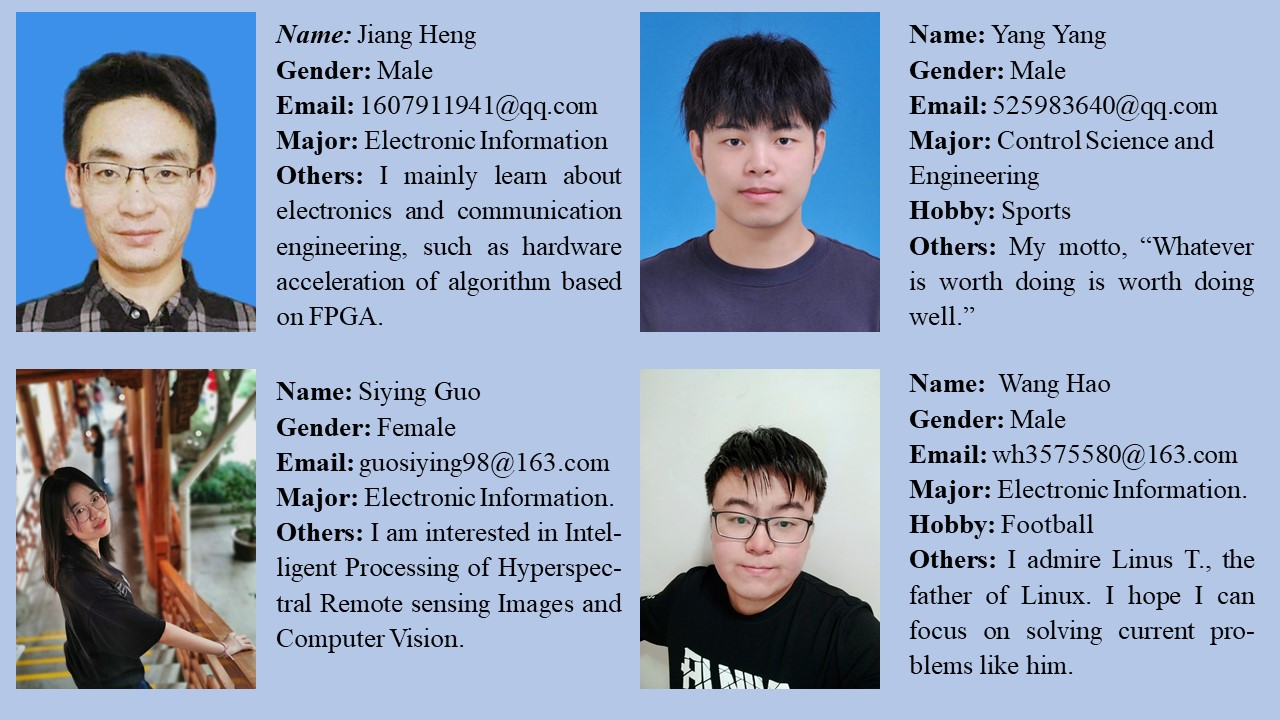
\includegraphics[width=17cm]{member.jpg}
\end{figure}

\section{{\LARGE About our team}}
Common goals and clear division of labor between teams are essential. On the one hand, our majors are different, and on the other hand, everyone has a certain aspect of knowledge. We will help each other and try our best to get things done.\\
As the course progresses, our homepage will be updated.
\end{document}

